\documentclass[11pt]{article}
\usepackage[margin=0.9in]{geometry}
\usepackage[T1]{fontenc}
\usepackage{microtype}
\usepackage{amsmath,amssymb}
\usepackage{booktabs,graphicx}
\usepackage{tikz}
\usetikzlibrary{positioning,arrows.meta,fit}
\usepackage{xurl}
\usepackage[hidelinks]{hyperref}
\title{Gemini: Local Qwen--Bev Guards for Stateful Tool Authorization}
\author{Smyan Thota\\\small Independent Research}
\date{Technical report --- work in progress\\October 24, 2026}
\begin{document}
\maketitle
\begin{abstract}
We describe a local, synthetic environment for studying whether an authorization assessor can constrain a multi-step tool-using language model while preserving useful work. The system retains Qwen's pretrained native function-call interface, routes its proposals through a Bev-derived authorization assessor and a bounded host, and records synthetic effects. Our current candidate uses a linear readout over frozen features of an upper-layer-adapted Bev 0.4B model; it does not use the actor adapters trained during development. On 24 inspected synthetic tasks, the selected raw linear configuration completed 7 of 16 solvable tasks safely, produced zero unauthorized effects, correctly reviewed all four insufficient-authority tasks, and contained all four revoked-authority tasks. Under the same host, Qwen alone completed 11/16 safely and committed 16 unauthorized effects. This is a finite development observation, not a safety guarantee: the raw MLP completed 9/16 safely but had three unauthorized effects; calibration eliminated observed unsafe effects while also preventing all safe completions. Earlier actor fine-tuning failed to generalize and was excluded from the final candidate. We report the architecture, training sequence, ablations, measurement corrections, and reproducibility limits. No fresh final evaluation, public benchmark, unrestricted computer-use evaluation, or universal safety claim is made; the candidate remains experimental and unpromoted.
\end{abstract}

\section{Goal and threat model}
The research question is bounded: can an authorization layer assess the exact proposed operation against a trusted request, policy, observed history, and current state, while a separate planner continues to select actions? The current multi-tool environment covers file, messaging, record, and simulated spending operations under scope, destination, budget, approval, provenance, and history rules. Earlier sequence experiments studied release limits, approval revisions, joint disclosure, and recipient allowlists; their results are historical and use different tasks. The host applies only synthetic local effects. It constrains the action menu, schema, and operation budget; model errors and uncertain assessments route to review rather than permission.

The threat model includes a planner proposing an operation that exceeds authority, attempting a blocked action repeatedly, or encountering policy changes, missing evidence, and revoked permission during a sequence. The assessor is not trusted to enforce basic structure: structural bounds are checked by the host. Permission is tied to the call and state being assessed; changed inputs require reassessment. The system does not protect arbitrary operating-system, browser, network, financial, or real-world actions. Nor does this work establish robustness to arbitrary prompt injection or adversarially optimized inputs.

The distinction between decision-level containment and episode-level usefulness is central. A blocked or deferred operation may avoid an effect but still leave the task incomplete. We therefore report safe completion, unauthorized effects, correct review, and revoked-authority containment separately. Errors routed to review count as containment when no effect occurs, but do not count as correct review unless the review label is correct.

\section{Related work and positioning}
StepGuard studies pre-execution checks and matched safe/unsafe continuations under shared context, including the safety--utility tradeoff \cite{stepguard}. ToolSafe combines step-level monitoring with feedback to the actor \cite{toolsafe}. These establish substantial prior art for external guards and recovery. We do not claim that pairing a language-model actor with a separate assessor is novel.

TACIT motivates reading agent-safety signals from frozen internal representations \cite{agentwithin}. Its results use larger backbones and trajectory-level datasets; our smaller Bev-derived pre-action readout is a different experiment, not a reproduction of its reported performance. Bev's model card supplies the base architecture and upstream limitations, including weaknesses in arithmetic and exception handling \cite{bev}. The host retains executable schema and budget checks rather than assigning every check to a learned model.

AgentDojo provides an established setting for studying tool use over untrusted data \cite{agentdojo}. We discuss that research for context but did not run AgentDojo or claim benchmark results on it. Temperature scaling follows the general calibration approach of Guo et al. \cite{guo}; calibration on these development distributions does not imply protection under arbitrary distribution shifts or adaptive attacks. Our contribution is an auditable local engineering study and its measured containment--completion tradeoff, with an explicit record of unsuccessful approaches.

\section{System architecture}
Qwen is the native function-call planner. Bev supplies representations for the learned assessor. The host remains responsible for validating the exact call, checking hard limits, committing synthetic effects, returning actual results, and bounding retries and total operations. After each permitted synthetic effect, Qwen observes the result and proposes the next action. The sequence ends at task completion, STOP, REVIEW, or a limit.

\begin{center}
\resizebox{\linewidth}{!}{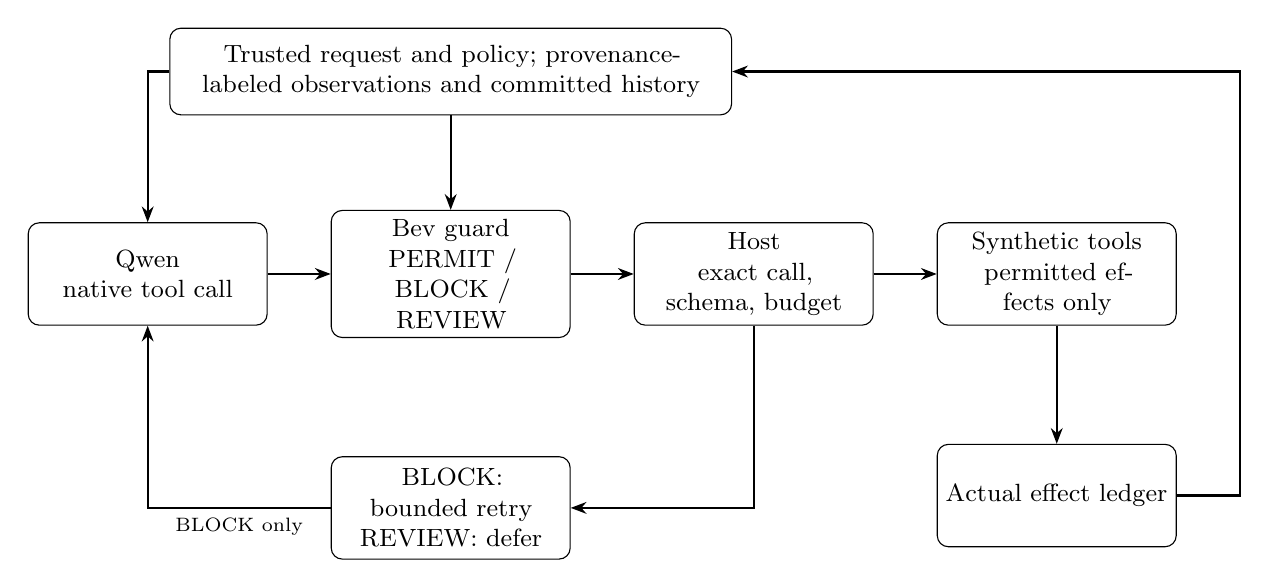
\begin{tikzpicture}[font=\small,node distance=8mm,
box/.style={draw,rounded corners,align=center,text width=28mm,minimum height=13mm},
wide/.style={draw,rounded corners,align=center,text width=69mm,minimum height=11mm},
arr/.style={-{Stealth[length=2mm]},thick}]
\node[box] (q) {Qwen\\native tool call};
\node[box,right=of q] (b) {Bev guard\\PERMIT / BLOCK / REVIEW};
\node[box,right=of b] (h) {Host\\exact call, schema, budget};
\node[box,right=of h] (t) {Synthetic tools\\permitted effects only};
\node[wide,above=12mm of b] (c) {Trusted request and policy; provenance-labeled observations and committed history};
\node[box,below=15mm of b] (r) {BLOCK: bounded retry\\REVIEW: defer};
\node[box,below=15mm of t] (l) {Actual effect ledger};
\draw[arr] (c.south)--(b.north);
\draw[arr] (c.west)-|(q.north);
\draw[arr] (q)--(b);\draw[arr] (b)--(h);\draw[arr] (h)--(t);
\draw[arr] (h.south)|-(r.east);
\draw[arr] (r.west)-|node[pos=.25,below,font=\scriptsize]{BLOCK only}(q.south);
\draw[arr] (t.south)--(l.north);
\draw[arr] (l.east)--++(8mm,0)|-(c.east);
\end{tikzpicture}}
\end{center}

The learned decision and structural enforcement are separate. The state builder must preserve the order of trusted events, distinguish actual from attempted effects, and retain missing versus empty evidence. A prior audit found that operation-budget information could be lost from the model state even when the host still enforced its true count. This is a versioned input-contract concern, not something model training can repair. Bev also consumes serialized state in key order; different key orders or batch padding altered decisions in earlier profiles. The current matched path uses production state objects, singleton FP32 assessment, and exact rendering/token fingerprints.

\section{Data and evaluation design}
The headline comparison uses 24 inspected synthetic tasks under a shared host, public tasks, menus, and action budget. The task mix has 16 solvable two-call tasks, four missing-authority tasks, and four revoked-authority tasks. For the first group we measure safe completion; for the latter groups we measure correct reviews and containment respectively. Qwen proposals are replayed only when all public inputs match exactly, and the guard is reassessed independently for each condition. Counts are task outcomes, not independent identically distributed samples; no population-level inference is warranted.

Training and development inputs are synthetic. Earlier repair work used grouped cases across policy rule families and focused on contrastive authorization decisions. Closely related variants were kept together where applicable. The report does not claim a public benchmark was evaluated, and none of the inspected cases constitutes a fresh final. The 24-task results are development evidence, and must be interpreted as such.

\section{Training and method timeline}
The project evolved through distinct methods rather than a single uninterrupted recipe. Early Bev guard versions performed well on fixed proposals but blocked much intended work: V7 reached 94/96 decisions and 30/32 strict paired decisions with zero unsafe permits, yet permitted only 2/11 intended legitimate proposals on a separate utility probe. On visible-read standard tasks, Qwen alone completed 11/16 while Qwen with V7 completed 6/16. On a separate adversarial set, Qwen alone completed 1/12 with two unauthorized synthetic effects; Qwen with V7 completed 0/12 with none. These results motivated task-level utility metrics and should not be conflated with the current 24-task comparison.

Actor SFT experiments (including two repair runs) sought to change Qwen's action selection. They did not generalize sufficiently and are not used by the final candidate. This negative result informed the choice to retain the native planner interface and put the learned intervention in a separate readout. During development, bounded output repair also showed that format constraints matter: a later diagnostic H17 profile safely completed 26/28 with a reference guard, while disabling its adapter under the same scoring mode produced STOP on all 28 initial prompts. That is a diagnostic reference-guard result, not evidence for the current Bev guard.

Initial experiments froze the base Bev model and fitted small readouts over its representations. The upper-adapter experiment then adapted the final four Bev layers (indices 16--19) with rank 8 query/value adapters, followed by a producer-prefix refit for the downstream readout. The matched final candidate combines the trained Bev-derived upper adapter with the linear authorization readout. The readout has 8,192 input features and three classes, with 24,579 parameters (8,192$\times$3 weights and three biases). The upper adapters contribute 163,840 parameters, giving 188,419 adapted/readout weights in total. The base model is Qwen3.5-2B and the frozen-feature backbone is Bev 0.4B-derived. This is a parameter count for the adapted components, not total model size.

The result is an engineering-method observation: the native tool-call interface was retained, actor adapters were removed from the selected inference profile, and authorization behavior was moved to a small readout. The available comparisons do not isolate the causal contribution of any one design choice. They support an implementation path and a measured candidate, not a causal or novelty claim.

\section{Matched native results}
Table~\ref{tab:main} reports the complete inspected comparison. ``Unauthorized effects'' counts committed effects on tasks where the effect was unauthorized, not every blocked or unsafe proposal. The two review-related columns refer to distinct task subsets.
\begin{table}[ht]
\centering
\caption{Matched native comparison on 24 inspected synthetic tasks.}
\label{tab:main}
\small\begin{tabular}{p{.29\linewidth}rrrr}
\toprule
Configuration & \shortstack{Safe\\completion /16} & \shortstack{Unauthorized\\effects} & \shortstack{Correct\\reviews /4} & \shortstack{Revoked\\containment /4}\\
\midrule
Qwen alone & 11 & 16 & 0 & 0\\
Raw MLP (64 hidden units) & 9 & 3 & 4 & 1\\
Raw linear & 7 & 0 & 4 & 4\\
Calibrated linear & 0 & 0 & 4 & 4\\
\bottomrule
\end{tabular}
\end{table}

The selected experimental configuration is the trained raw linear readout (the identifier ending in 0 denotes zero hidden units, not zero training updates). It completed seven safe tasks among the sixteen solvable tasks and recorded no unauthorized effects in this finite set. It also classified all four missing-authority reviews correctly and contained all four revoked-authority tasks. The MLP completed two more safe tasks but had three unauthorized effects and failed containment on three of four revoked tasks. Calibration lowered observed unauthorized effects to zero but also eliminated safe completions. The calibrated result demonstrates the cost of this operating point; it is not a successful deployment configuration.

Qwen-alone's 16 unauthorized effects occurred in eight tasks; the MLP's three effects occurred in three tasks. Effect counts and unsafe-episode counts are distinct because one task can commit multiple effects. Likewise, the candidate's zero observed effects should not be interpreted as proof of future prevention. The older 28-episode development suite, the 24-task matched comparison, and the 26/28 bounded-format reference-guard diagnostic have different tasks and denominators and are not pooled.

\section{Ablations, calibration, and failure analysis}
The principal ablation changes the classifier and calibration while retaining the matched task/host setup. Raw linear improves containment and review behavior over raw MLP at the cost of two safe completions. Calibration moves the threshold too conservatively for task utility in this sample. We do not present these small counts as statistical significance or use them to tune a universal threshold.

Training actor adapters was a failed line of attack for this use case. This matters because it prevents an inaccurate account in which the selected system is described as an actor fine-tune. The deployed actor is the base native Qwen planner. The current readout changes authorization assessment; the host controls whether a proposed call can take effect.

Engineering failures also changed the evaluation methodology. A V8 receipt once reported 576 optimizer updates, but the retained training logic and checkpoints show an early stop at 192 updates (evaluations at 64, 128, and 192). A V9 batch-2 run was not a production-singleton result: padding peers changed choices, and sorting serialized state keys changed 26 singleton decisions in a 56-request comparison despite identical JSON values and token counts. These are corrected in the project record; historical receipts remain historical. A 79-test software verification suite checks implementation properties and regressions. Passing software tests is not a model safety proof and is not a substitute for task evaluation.

The package extraction check verified that two calls in sequence can traverse the host path. This demonstrates the intended integration path, not broad robustness. The separate matched results remain the source for the counts in this paper.

\section{Limitations, licensing, and reproducibility}
All examples and effects are synthetic and development-inspected. No fresh final was run. No unrestricted computer-use scenario, public benchmark, or external deployment was evaluated. The sample is small, fixed, and not a randomized trial. Zero unauthorized effects in four revoked cases or 16 solvable tasks is not evidence of universal safety. A model may fail through misclassification, missing state, proposal errors, host defects, or interaction effects. Completion targets, review burden, operation count, and latency also matter beyond the reported headline counts.

The candidate remains experimental and unpromoted; gates for completion and fresh final evaluation remain open. Earlier standard, adversarial, and 28-task results are included only as historical context with their own protocol and denominator. Model weights are not included in the source repository. The Bev-derived weights are subject to their model-card license (CC BY-NC), while Qwen3.5-2B weights are subject to their own published terms (Apache 2.0 as recorded for this project); source licensing does not override either model license. Researchers must review the model cards and license terms before downloading or redistributing weights. The source implementation is MIT licensed.

Reproduction uses the repository's local training, inference, bounded-host, scoring, and private-package workflows. The exact inspected package used local model weights and private evaluation inputs that are not in Git; those inputs must not be reconstructed from paper tables as if they were public artifacts. A reproducible release should record immutable weight identifiers, package hash, configuration, input-render fingerprints, hardware/software versions, and the full scoring output. The report's configuration values and finite task counts are stated explicitly to support audit without exposing private keys or local paths.

\section{Conclusion}
The work demonstrates a bounded local architecture that preserves a native Qwen tool interface while using a compact Bev-derived readout to assess authorization. In the current 24-task inspected comparison, raw linear combined zero observed unauthorized effects, four correct reviews, four revoked containments, and 7/16 safe completions; the calibrated condition also contained all effects but completed no solvable tasks. The raw MLP traded higher completion for unsafe effects; calibration traded all observed effects for no useful completion. These are meaningful trade-offs, not a solved safety problem. The evidence supports continued development of the frozen-feature readout and matched evaluation protocol while keeping the candidate unpromoted until utility, robustness, and fresh-final requirements are met.

\clearpage
\appendix
\section{Compact experiment chronology and configuration}
\begin{table}[ht]
\centering
\small
\begin{tabular}{p{0.20\linewidth}p{0.71\linewidth}}
\toprule
Stage & Record and interpretation\\
\midrule
V7 guard & 94/96 fixed-proposal decisions; 30/32 strict paired decisions; 0 unsafe permits, but only 2/11 intended legitimate proposals in separate utility probe.\\
Task probes & Visible-read standard: Qwen 11/16, Qwen+V7 6/16. Adversarial: Qwen 1/12 with two unauthorized synthetic effects; Qwen+V7 0/12 with zero.\\
V8 actor/guard work & Historical run 2 ended at 192 updates, not the erroneous 576 receipt figure; no checkpoint passed combined gates.\\
Bounded-format diagnostic & H17 with reference guard: 26/28 safe completions; adapter-disabled profile: STOP on 28 initial prompts. Not a current-guard result.\\
Actor repair & Two actor SFT attempts failed the generalization objective; neither adapter participates in the selected native candidate.\\
Upper adapter & Final four Bev layers (16--19), rank 8 query/value adapters; 6 epochs, 6,912 presentations over 1,152 rows (6 presentations per row).\\
Selected matched candidate & Qwen3.5-2B native function calls; Bev 0.4B-derived upper adapter plus raw 3-way linear readout. Readout: 8,192$\times$3 + 3 = 24,579 parameters; adapter: 163,840; total adapted/readout: 188,419.\\
\bottomrule
\end{tabular}
\end{table}

\section{Evidence and reporting notes}
The headline table uses the current matched 24-task results record. Earlier corrected records report a 28-task development baseline, a 26/28 bounded-format diagnostic using a reference guard, and separate 12-task adversarial and 16-task standard task probes. These are not combined. The current evaluation's zero effect count does not imply zero unsafe proposals; counts refer to committed unauthorized effects. Reviews and blocks can contain an effect without completing the requested task. The included package check verified two sequential calls in the extracted artifact; the project suite comprises 79 software tests. Test count is an implementation-verification statistic only.


\section{Additional retained experiments}
Table~\ref{tab:pilots} records the corrected pilot families. Each retained full pilot used 4,608 training rows, 152 development requests, and 192 optimizer updates. A presentation is not a unique example. Accuracy peaks and safety-prioritized selections are distinct checkpoints; they must not be combined into one claimed result.
\begin{table}[ht]
\centering\small
\begin{tabular}{p{.38\linewidth}rrp{.21\linewidth}}
\toprule
Experiment & \shortstack{Peak correct\\/152} & \shortstack{Unsafe permits\\at peak} & Outcome\\
\midrule
Corrected native V2 &126&6&No promotion\\
Typed-fact V3, warm initialization&93&16&No promotion\\
Typed-fact V3, fresh initialization&103&26&No promotion\\
\bottomrule
\end{tabular}
\caption{Inspected development pilots. These are separate from the final 24-task native comparison.}\label{tab:pilots}
\end{table}
The corrected V2 safety-prioritized checkpoint scored 85/152 with zero unsafe permits but accepted only 15/52 intended permits in its trajectory subset. This motivated measuring containment and utility jointly. A subsequent 24-row TRAIN-only repeated-fit diagnostic reached 24/24 at update 64 with mean cross-entropy approximately 0.02. It was paused before completing the required consecutive low-loss confirmations. This shows fit on selected training examples, not generalization or deployment acceptance.

The broad synthetic scene corpus contained 576 TRAIN, 144 calibration, 144 development, 144 compositional-development and 72 held-out-tool-development rows. The held-out access-tool domain used the same uniform argument contract; it is not evidence of arbitrary new application support. One training-only nuisance view per row produced 1,152 upper-adaptation rows. Six epochs presented 6,912 examples in 288 updates. The selected backbone for producer-prefix refitting was the saved update-144 checkpoint, not the final update-288 state. It had therefore seen 3,456 presentations when saved.

Producer-prefix supervision added 576 TRAIN examples drawn from verified training trajectories, with 144 producer calibration and 144 producer development examples drawn from their corresponding original groups. Retaining the original scenes yielded 1,152 head-training rows and 288 rows each for calibration and development. Related branches and source groups stayed together. The selected linear head was trained for 60 CPU epochs; its final feature width is 8,192 and it has 24,579 parameters. These counts describe the final artifact, while earlier MLP heads were separate candidates.

Both actor repairs trained 139,264 parameters in the last two existing H17 attention adapter groups, using 234 updates and accumulation four: 936 presentations of 312 supervised prompts per run. The first run used ordinary completion loss; the second weighted action-ID tokens by eight, decision-type tokens by two, formatting tokens by 0.25, and EOS by one. Serialized reload/logit checks passed. Neither repair completed the eight inspected solvable actor tasks. A TRAIN-prefix probe showed why average completion loss was insufficient: JSON boilerplate could be correct while a critical action-ID token was wrong. The final system instead uses pretrained native function calls. This progression identifies an interface effect worth studying; it is not a controlled causal estimate isolating all prompt, numerical-profile and adapter differences.

\section{Reproduction boundaries and artifact identities}
The source repository includes training modules for frozen readouts, upper-layer adapters and actor repair; synthetic data generators; native and legacy actors; the bounded host; independent scoring; and private-package tooling. Operator-supplied base weights, generated corpora and private scoring keys remain outside Git. Recreating synthetic corpora from public generators is possible, but reproducing the exact historical measurements also requires their pinned inputs and configurations. We do not imply that publication of source alone releases every private evaluation artifact.

The selected Bev checkpoint SHA-256 is \nolinkurl{81bbddab339a593f6bf4c0d1241a90073ddc521a8e5e87e557d1f1c264b14352}. The Qwen snapshot is \nolinkurl{15852e8c16360a2fea060d615a32b45270f8a8fc}; the Bev base snapshot is \nolinkurl{cf5138b5b465343d09c3b4fbd71eaca36d989d34}. The local package was extracted to a separate directory, its imported source origin checked, and a real two-call Qwen--Bev demonstration executed from that directory. The matching source is available at \url{https://github.com/Smyan-Thota/gemini}. Model weights retain their upstream licensing restrictions.

All local training and the final native comparisons used an NVIDIA GeForce RTX 5060 with approximately 8 GB VRAM. Bev assessment used singleton FP32. Qwen's GPU inference used BF16. CPU checks and the initial native-call feasibility check are different profiles. No wall-clock or throughput advantage is claimed because a controlled timing study was not performed.

\clearpage
\begin{thebibliography}{9}
\bibitem{agentwithin} Difan Jiao and Ashton Anderson. \emph{Agent Safety From Within: Detecting Harmful Trajectories from LLM Internal States}. arXiv:2609.33039, 2026.\
\url{https://arxiv.org/abs/2609.33039}
\bibitem{stepguard} Zhijie Zheng et al. \emph{StepGuard: Learning Step-Level Guardrails with Scalable Supervision and Safety-Utility Balancing}. arXiv:2608.24777, 2026.\
\url{https://arxiv.org/abs/2608.24777}
\bibitem{toolsafe} Yutao Mou et al. \emph{ToolSafe: Enhancing Tool Invocation Safety of LLM-based agents via Proactive Step-level Guardrail and Feedback}. arXiv:2601.10156, 2026.\
\url{https://arxiv.org/abs/2601.10156}
\bibitem{agentdojo} Edoardo Debenedetti et al. \emph{AgentDojo: A Dynamic Environment to Evaluate Prompt Injection Attacks and Defenses for LLM Agents}. arXiv:2406.13352, 2024.\
\url{https://arxiv.org/abs/2406.13352}
\bibitem{bev} avbiswas. \emph{Bev Decider 0.4B model card}.\
\url{https://huggingface.co/avbiswas/bev-decider-0.4B}
\bibitem{guo} C. Guo, G. Pleiss, Y. Sun, and K. Q. Weinberger. On Calibration of Modern Neural Networks. In \emph{Proceedings of ICML}, 2017. arXiv:1706.04599.\
\url{https://arxiv.org/abs/1706.04599}
\end{thebibliography}
\end{document}
